\documentclass[10pt, a4paper, onecolumn, oneside, titlepage, openany]{book}

\usepackage[T1]{fontenc}
\usepackage[utf8]{inputenc}
\usepackage{titlesec} % chapter on line with text
\usepackage{fancyhdr}
\usepackage{hyperref}
\hypersetup{
    colorlinks=true,
    linkcolor=blue, %\ref{}
    filecolor=magenta, % \href{run:./file.txt}{File.txt}
    urlcolor=cyan, % \href{http://www.overleaf.com}{Link}
    pdftitle={Cisco CCNA}
    pdfpagemode=FullScreen,
    }
\usepackage{menukeys}
\usepackage{fancyvrb}

% table formatting
\setlength{\arrayrulewidth}{0.5mm} % border
\setlength{\tabcolsep}{18pt} % space from border (X axis)
\renewcommand{\arraystretch}{1.5} % space from border (Y axis)
\usepackage[format=hang,font=small,labelfont=bf]{caption} % bold table caption

% chapter formatting
\renewcommand{\chaptername}{}
\titleformat{\chapter}[hang]{\normalfont\huge\bfseries}{\chaptertitlename\ \thechapter.}{1em}{}

% decorative lines:
\renewcommand{\headrulewidth}{2pt}
\renewcommand{\footrulewidth}{2pt}
\pagestyle{fancy}
\fancyhf{}
    \chead{\leftmark}
    \cfoot{\thepage}
\fancypagestyle{plain}{
\fancyhf{}
    \chead{\leftmark}
    \cfoot{\thepage}
}

% verbatim formatting
\definecolor{device}{RGB}{0, 100, 200}
\definecolor{command}{RGB}{41, 182, 0}
\definecolor{nocommand}{RGB}{222, 0, 0}
\definecolor{showcommand}{RGB}{255, 80, 0}
\definecolor{warncommand}{RGB}{255, 80, 0}
\definecolor{root}{RGB}{222, 0, 0}
\definecolor{user}{RGB}{0, 150, 0}
\definecolor{dir}{RGB}{0, 100, 200}
\definecolor{file}{RGB}{77, 187, 101}
\definecolor{block}{RGB}{255, 80, 0}
\definecolor{comment}{RGB}{0, 182, 182}
\definecolor{background}{RGB}{240, 240, 240}
\renewcommand{\FancyVerbFormatLine}[1]{\colorbox{background}{#1}}


\title{\textbf{Linux Artix}}
\author{AISK11}
\date{March 2022}

\begin{document}
\maketitle
\tableofcontents


\chapter{System Info}
\section{System Hardware}
\begin{table}[h!]
\centering
\begin{tabular}{|c|c|}
    \hline
    \textbf{Hardware} & \textbf{Value} \\
    \hline
    CPU architecture & amd64\\
    CPU vendor & intel\\
    Motherboard & UEFI\\
    Hard Drive & NVMe\\
    WiFi & iwlwifi\\
    GPU & Intel + Nvidia\\
    \hline
\end{tabular}
\caption{System hardware overview.}
\label{table:1}
\end{table}

\section{System Software}
\begin{table}[h!]
\centering
\begin{tabular}{|c|c|}
    \hline
    \textbf{Hardware} & \textbf{Value} \\
    \hline
    RAID & no\\
    LVM & no (btrfs)\\
    Encryption & LUKS\\
    Root filesystem & btrfs\\
    SWAP & 4GB (file)\\
    Bootloader & rEFInd\\
    Init & runit\\
    Virtualization & Xen\\
    \hline
\end{tabular}
\caption{System software overview.}
\label{table:2}
\end{table}


\chapter{Download}
\section{Download Artix ISO}
\begin{enumerate}
    \item \textbf{Download Artix ISO}
    \begin{itemize}
        \item \textbf{Artix download page:}
\newline \url{https://artixlinux.org/download.php}
        \item \textbf{Select install file:}
\newline \menu[,]{Official ISO images, base, artix-base-runit-20220123-x86\_64.iso}
    \end{itemize}
    \item \textbf{Verify download: @TODO}
\end{enumerate}

\section{USB preparation}
\begin{enumerate}
    \item \textbf{Unmount USB FS!}
    \item \textbf{Flash image to USB:}
\begin{Verbatim}[commandchars=\\\{\}]
\textcolor{root}{root#} \textcolor{command}{dd} if=<\textcolor{file}{./artix-base-runit-<YYYYMMDD>-x86_64.iso>.iso}> of=<\textcolor{block}{/dev/sdX}>
[conv=fsync] [bs=4M] [status=progress] && \textcolor{command}{sync}
\end{Verbatim}
\end{enumerate}

\section{Boot Live Installer}
\subsection{Secure Boot}
Make sure, that Secure Boot is disabled!
\begin{enumerate}
    \item \textbf{During POST press key to access BIOS/UEFI:}
\newline \href{https://techofide.com/blogs/boot-menu-option-keys-for-all-computers-and-laptops-updated-list-2021-techofide/}{https://techofide.com/blogs/boot-menu-option-keys-for-all-computers-and-laptops-updated-list-2021-techofide/}
    \item \textbf{Disable Secure Boot}
    \item \textbf{Poweroff/Restart}
\end{enumerate}
\subsection{Boot}
\begin{enumerate}
    \item \textbf{Plug in flashed USB}
    \item \textbf{During POST press key to access Boot Menu:}
\newline \href{https://techofide.com/blogs/boot-menu-option-keys-for-all-computers-and-laptops-updated-list-2021-techofide/}{https://techofide.com/blogs/boot-menu-option-keys-for-all-computers-and-laptops-updated-list-2021-techofide/}
    \item \textbf{Select USB entry (UEFI)}
\end{enumerate}


\chapter{Pre-Installation}
\section{Login}
\begin{itemize}
    \item \textbf{Login to live environment:}
\begin{Verbatim}[commandchars=\\\{\}]
> artix
> artix
\end{Verbatim}
    \item \textbf{Access root:}
\begin{Verbatim}[commandchars=\\\{\}]
\textcolor{user}{user\$} \textcolor{command}{sudo} passwd root
> <NEW_ROOT_PWD>
> <NEW_ROOT_PWD (VERIFY)>
\textcolor{user}{user\$} \textcolor{command}{su} -
\end{Verbatim}
\end{itemize}

\section{Verify UEFI}
\begin{itemize}
    \item \textbf{UEFI is used if following directory exists:}
\newline \textbf{\textcolor{dir}{/sys/firmware/efi/}}
    \item \textbf{Verify via kernel:}
\begin{Verbatim}[commandchars=\\\{\}]
\textcolor{root}{root#} \textcolor{command}{dmesg} | \textcolor{command}{grep} -i efi
\end{Verbatim}
\end{itemize}

\section{Connect To The Internet @TODO}
\begin{itemize}
    \item \textbf{Ethernet}

    \item \textbf{WiFi}
\end{itemize}

\section{Time Sync @TODO}

\section{Install additional software}
\begin{enumerate}
    \item \textbf{Synchronize database:}
\begin{Verbatim}[commandchars=\\\{\}]
\textcolor{root}{root#} \textcolor{command}{yes} | \textcolor{command}{pacman} -Syy
\end{Verbatim}
    \item \textbf{Install parted:}
\begin{Verbatim}[commandchars=\\\{\}]
\textcolor{root}{root#} \textcolor{command}{yes} | \textcolor{command}{pacman} -S parted
\end{Verbatim}
\end{enumerate}

\section{Check Disk Sectors}
\subsection{Theory}
\begin{itemize}
    \item \textbf{Sector:} smallest unit size on disk. 512 or 4096 bytes (Advanced Format). 4096 Advanced Format disks have usually 512-byte conversion firmware.
    \item \textbf{Block:} allocation size the FS uses. Cannot be smaller than size of the sector. Can be group of sectors (4096b: 8 x 512b sectors).
    \begin{itemize}
        \item \textbf{512b =} good for lot of small files. More blocks = more metadata.
        \item \textbf{4096b =}  good for larger files, less metadata. Waste if there are mostly small files.
    \end{itemize}
\end{itemize}
\subsection{Disk Information}
\begin{itemize}
    \item \textbf{Find disks (block devices):}
\begin{Verbatim}[commandchars=\\\{\}]
\textcolor{user}{user\$} \textcolor{command}{lsblk} [-ap | -apf]
\textcolor{root}{root#} \textcolor{command}{fdisk -l} [\textcolor{block}{/dev/sdX}]
\textcolor{root}{root#} \textcolor{command}{gdisk -l} <\textcolor{block}{/dev/sdX}>
\textcolor{root}{root#} \textcolor{command}{blkid}
\end{Verbatim}
    \item \textbf{Get raw disk info:}
    \begin{itemize}
        \item \textbf{Get disk physical sector size:}
\begin{Verbatim}[commandchars=\\\{\}]
\textcolor{root}{root#} \textcolor{command}{blockdev} [-v] --getpbsz <\textcolor{block}{/dev/sdX[Y]}>
\end{Verbatim}
        \item \textbf{Get disk logical sector size (usually 512):}
\begin{Verbatim}[commandchars=\\\{\}]
\textcolor{root}{root#} \textcolor{command}{blockdev} [-v] --getss <\textcolor{block}{/dev/sdX[Y]}>
\end{Verbatim}
        \item \textbf{Disk size in bytes:}
\begin{Verbatim}[commandchars=\\\{\}]
\textcolor{root}{root#} \textcolor{command}{blockdev} [-v] --getsize64 <\textcolor{block}{/dev/sdX[Y]}>
\end{Verbatim}
    \item \textbf{Check if disk is readonly (1 = ro, 0 = rw):}
\begin{Verbatim}[commandchars=\\\{\}]
\textcolor{root}{root#} \textcolor{command}{blockdev} [-v] --getro <\textcolor{block}{/dev/sdX[Y]}>
\end{Verbatim}
    \end{itemize}
    \item \textbf{See partitions:}
\begin{Verbatim}[commandchars=\\\{\}]
\textcolor{root}{root#} \textcolor{command}{parted} -s <\textcolor{block}{/dev/sdX}> (p)rint [free]
\end{Verbatim}
\end{itemize}
\subsection{Check Disk For Bad Sectors}
\begin{enumerate}
    \item \textbf{Unmount FS!}
    \item \textbf{Check disk for bad blocks:}
\begin{Verbatim}[commandchars=\\\{\}]
\textcolor{root}{root#} \textcolor{command}{badblocks} [-b 4096] [-w [-t 0xaa]] [-v] [-s]
<\textcolor{block}{/dev/sdX[Y]}> | \textcolor{command}{tee} -a <\textcolor{file}{OUTPUT_FILE}>
\end{Verbatim}
\end{enumerate}


\chapter{Installation}
\section{Disk Partitioning}
\begin{figure}[ht]
    \begin{center}
        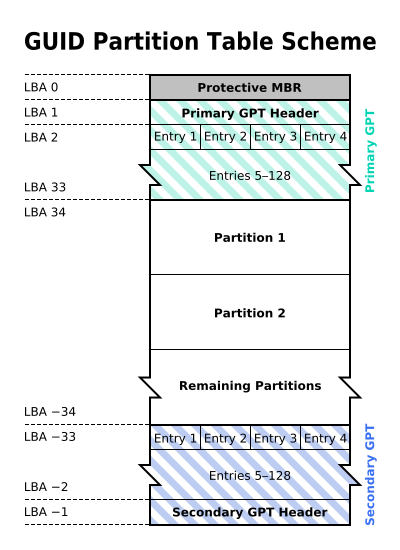
\includegraphics[width=40mm]{./src/img/gpt1.png}
        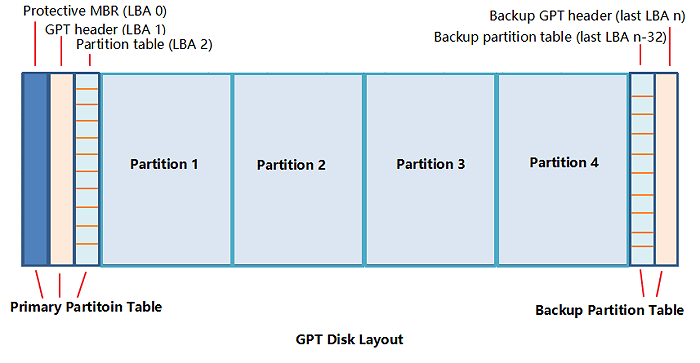
\includegraphics[width=75mm]{./src/img/gpt2.png}
        \caption{GPT Partition Table.}
        \label{fig:1}
    \end{center}
\end{figure}
\subsection{Partition Table}
\begin{enumerate}
    \item \textbf{Unmount FS!}
    \item \textbf{Create GPT partition table:}
\begin{Verbatim}[commandchars=\\\{\}]
\textcolor{root}{root#} \textcolor{command}{parted} -s <\textcolor{block}{/dev/sdX}> mktable gpt
\end{Verbatim}
\end{enumerate}
\subsection{Basic Partitions}
\begin{enumerate}
    \item \textbf{Enter cfdisk:}
\begin{Verbatim}[commandchars=\\\{\}]
\textcolor{root}{root#} \textcolor{command}{cfdisk} <\textcolor{block}{/dev/sdX}>
\end{Verbatim}
    \item \textbf{Create EFI partition (recommended 550 MiB):}
\begin{Verbatim}[commandchars=\\\{\}]
\textcolor{root}{cfdisk>} \textcolor{command}{n}
\textcolor{root}{cfdisk>} \textcolor{command}{550MiB}
\textcolor{root}{cfdisk>} \textcolor{command}{t}
\textcolor{root}{cfdisk>} \textcolor{command}{EFI System}
\end{Verbatim}
    \item \textbf{Create encrypted partition:}
\begin{Verbatim}[commandchars=\\\{\}]
\textcolor{root}{cfdisk>} \textcolor{command}{n}
\textcolor{root}{cfdisk>} \textcolor{command}{} (Enter)
\end{Verbatim}
    \item \textbf{Write changes:}
\begin{Verbatim}[commandchars=\\\{\}]
\textcolor{root}{cfdisk>} \textcolor{command}{W}
\textcolor{root}{cfdisk>} \textcolor{command}{yes}
\end{Verbatim}
    \item \textbf{Quit cfdisk:}
\begin{Verbatim}[commandchars=\\\{\}]
\textcolor{root}{cfdisk>} \textcolor{command}{Q}
\end{Verbatim}
    \item \textbf{Name partitions:}
\begin{Verbatim}[commandchars=\\\{\}]
\textcolor{root}{root#} \textcolor{command}{parted} -s <\textcolor{block}{/dev/sdX}> name 1 ESP
\textcolor{root}{root#} \textcolor{command}{parted} -s <\textcolor{block}{/dev/sdX}> name 2 LUKS
\end{Verbatim}
    \item \textbf{Format partitions:}
    \begin{enumerate}
        \item \textbf{ESP:}
\begin{Verbatim}[commandchars=\\\{\}]
\textcolor{root}{root#} \textcolor{command}{mkfs.fat} -F 32 <\textcolor{block}{/dev/sdX1}>
\textcolor{root}{root#} \textcolor{command}{fatlabel} <\textcolor{block}{/dev/sdX1}> <ESP>
\end{Verbatim}
        \item \textbf{LUKS:}
\begin{Verbatim}[commandchars=\\\{\}]
\textcolor{root}{root#} \textcolor{command}{cryptsetup} luksFormat --label <LUKS> <\textcolor{block}{/dev/sdX2}>
> YES
> <PASSWORD>
> <PASSWORD (VERIFY)>
\end{Verbatim}
    \end{enumerate}
\end{enumerate}
    \subsection{(Advanced LUKS Stuff)}
\begin{itemize}
    \item \textbf{Open LUKS:}
\begin{Verbatim}[commandchars=\\\{\}]
\textcolor{root}{root#} \textcolor{command}{cryptsetup} open --type luks <\textcolor{block}{/dev/sdX2}> <luks>
> <PASSWORD>
\end{Verbatim}
    \item \textbf{Close LUKS:}
\begin{Verbatim}[commandchars=\\\{\}]
\textcolor{root}{root#} \textcolor{command}{cryptsetup} close <luks>
\end{Verbatim}
    \item \textbf{LUKS header:}
    \begin{enumerate}
        \item \textbf{See LUKS header:}
\begin{Verbatim}[commandchars=\\\{\}]
\textcolor{root}{root#} \textcolor{command}{cryptsetup} luksDump <\textcolor{block}{/dev/sdX2}>
\end{Verbatim}
        \item \textbf{Make LUKS header backup:}
\begin{Verbatim}[commandchars=\\\{\}]
\textcolor{root}{root#} \textcolor{command}{cryptsetup} luksHeaderBackup <\textcolor{block}{/dev/sdX2}>
--header-backup-file <\textcolor{file}{FILE}>
\end{Verbatim}
        \item \textbf{Destroy LUKS header:}
\begin{Verbatim}[commandchars=\\\{\}]
\textcolor{root}{root#} \textcolor{command}{cryptsetup} luksErase <\textcolor{block}{/dev/sdX2}>
> YES
\end{Verbatim}
        \item \textbf{Restore LUKS header:}
\begin{Verbatim}[commandchars=\\\{\}]
\textcolor{root}{root#} \textcolor{command}{cryptsetup} luksHeaderRestore <\textcolor{block}{/dev/sdX2}>
--header-backup-file <\textcolor{file}{FILE}>
> YES
\end{Verbatim}
    \end{enumerate}
    \item \textbf{Passwords}
    \begin{itemize}
        \item \textbf{Change password:}
\begin{Verbatim}[commandchars=\\\{\}]
\textcolor{root}{root#} \textcolor{command}{cryptsetup} luksChangeKey <\textcolor{block}{/dev/sdX2}>
> <OLD_PASSWORD>
> <NEW_PASSWORD>
> <NEW_PASSWORD (VERIFY)>
\end{Verbatim}
    \end{itemize}
\end{itemize}
\subsection{Encrypted Partition}
\begin{figure}[ht]
    \begin{center}
        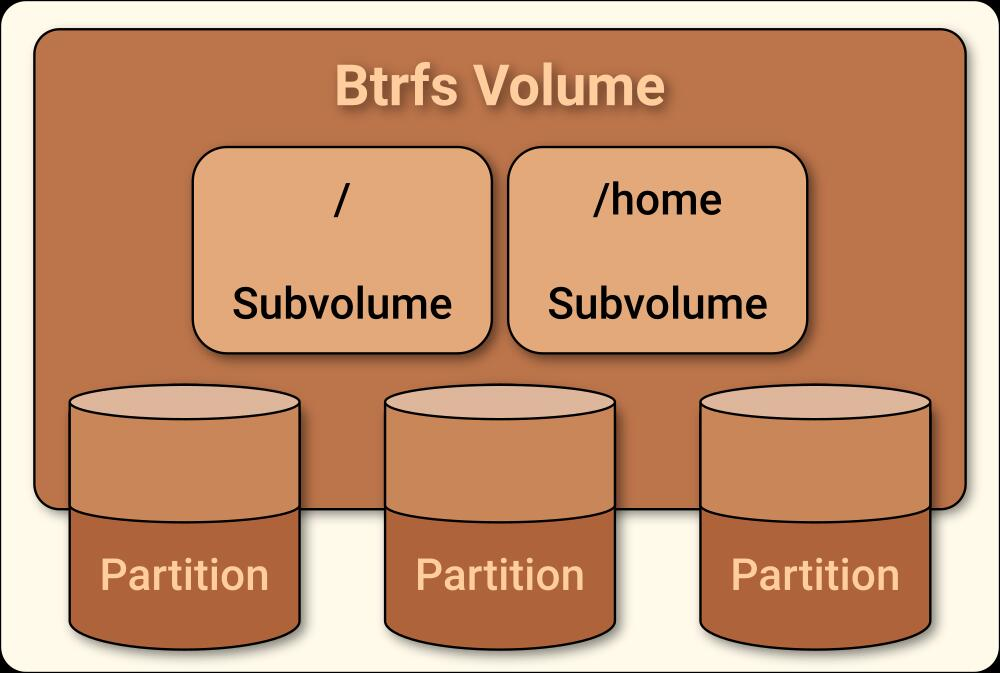
\includegraphics[width=75mm]{./src/img/btrfs.png}
        \caption{Btrfs structure.}
        \label{fig:2}
    \end{center}
\end{figure}
\begin{enumerate}
    \item \textbf{Open encrypted partition:}
\begin{Verbatim}[commandchars=\\\{\}]
\textcolor{root}{root#} \textcolor{command}{cryptsetup} open --type luks <\textcolor{block}{/dev/sdX2}> <luks-root>
> <PASSWORD>
\end{Verbatim}
    \item \textbf{Format root partition:}
\begin{Verbatim}[commandchars=\\\{\}]
\textcolor{root}{root#} \textcolor{command}{mkfs.btrfs} <\textcolor{block}{/dev/mapper/luks-root}>
\textcolor{root}{root#} \textcolor{command}{btrfs} filesystem label <\textcolor{block}{/dev/mapper/luks-root}> <LUKS-ROOT>
\end{Verbatim}
\end{enumerate}

\section{Base Artix Installation}
\begin{enumerate}
    \item \textbf{Create mount directory:}
\begin{Verbatim}[commandchars=\\\{\}]
\textcolor{root}{root#} \textcolor{command}{mkdir} <\textcolor{dir}{/mnt/artix/}>
\end{Verbatim}
    \item \textbf{Mount Artix:}
\begin{Verbatim}[commandchars=\\\{\}]
\textcolor{root}{root#} \textcolor{command}{mount} <\textcolor{block}{/dev/mapper/luks-root}> <\textcolor{dir}{/mnt/artix/}>
\end{Verbatim}
    \item \textbf{Install packages to new directory:}
\begin{Verbatim}[commandchars=\\\{\}]
\textcolor{root}{root#} \textcolor{command}{basestrap} <\textcolor{dir}{/mnt/artix/}> base
\end{Verbatim}
\end{enumerate}

\section{Chroot}
\begin{enumerate}
    \item \textbf{Mount all filesystems:}
\begin{Verbatim}[commandchars=\\\{\}]
\textcolor{root}{root#} \textcolor{command}{mount} -t proc \textcolor{dir}{/proc/} <\textcolor{dir}{/mnt/artix/proc/}>
\textcolor{root}{root#} \textcolor{command}{mount} --rbind \textcolor{dir}{/sys/} <\textcolor{dir}{/mnt/artix/sys/}>
\textcolor{root}{root#} \textcolor{command}{mount} --make-rslave <\textcolor{dir}{/mnt/artix/sys/}>
\textcolor{root}{root#} \textcolor{command}{mount} --rbind \textcolor{dir}{/dev/} <\textcolor{dir}{/mnt/artix/dev/}>
\textcolor{root}{root#} \textcolor{command}{mount} --make-rslave <\textcolor{dir}{/mnt/artix/dev/}>
\textcolor{root}{root#} \textcolor{command}{mount} --bind \textcolor{dir}{/run/} <\textcolor{dir}{/mnt/artix/run/}>
\textcolor{root}{root#} \textcolor{command}{mount} --make-slave <\textcolor{dir}{/mnt/artix/run/}>
\end{Verbatim}
    \item \textbf{Chroot:}
\begin{Verbatim}[commandchars=\\\{\}]
\textcolor{root}{root#} \textcolor{command}{chroot} <\textcolor{dir}{/mnt/artix/}> \textcolor{file}{/bin/bash}
\textcolor{root}{root#} \textcolor{command}{source} \textcolor{file}{/etc/profile}
\textcolor{root}{root#} \textcolor{command}{export} PS1="(chroot) \$\{PS1\}"
\end{Verbatim}
    \item \textbf{Mount boot partition:}
\begin{Verbatim}[commandchars=\\\{\}]
\textcolor{root}{(chroot) root#} \textcolor{command}{mount} <\textcolor{block}{/dev/sdX1}> \textcolor{dir}{/boot/}
\end{Verbatim}
\end{enumerate}

\section{Pacman Configuration}
\begin{enumerate}
    \item \textbf{Add additional Arch packages:}
\begin{Verbatim}[commandchars=\\\{\}]
\textcolor{root}{(chroot) root#} [\textcolor{command}{yes} |] \textcolor{command}{pacman} -S artix-archlinux-support
\end{Verbatim}
    \item \textbf{Pacman configuration:}
\newline File (\textbf{\textcolor{file}{/etc/pacman.conf}}):
\newline \url{https://github.com/AISK11/Artix/blob/main/configs/pacman/pacman.conf}
    \item \textbf{Synchronize new repos [and update]:}
\begin{Verbatim}[commandchars=\\\{\}]
\textcolor{root}{(chroot) root#} \textcolor{command}{pacman} -Syy[u]
\end{Verbatim}
\end{enumerate}

\section{Additional Packages}
\begin{itemize}
    \item \textbf{Text editor:}
\begin{Verbatim}[commandchars=\\\{\}]
\textcolor{root}{(chroot) root#} [\textcolor{command}{yes} |] \textcolor{command}{pacman} -S vim
\end{Verbatim}
    \item \textbf{Git:}
\begin{Verbatim}[commandchars=\\\{\}]
\textcolor{root}{(chroot) root#} [\textcolor{command}{yes} |] \textcolor{command}{pacman} -S git
\end{Verbatim}
    \item \textbf{Partitioning}
\begin{Verbatim}[commandchars=\\\{\}]
\textcolor{root}{(chroot) root#} [\textcolor{command}{yes} |] \textcolor{command}{pacman} -S parted
\end{Verbatim}
    \item \textbf{Filesystems:}
\begin{Verbatim}[commandchars=\\\{\}]
\textcolor{root}{(chroot) root#} [\textcolor{command}{yes} |] \textcolor{command}{pacman} -S dosfstools cryptsetup btrfs-progs
\end{Verbatim}
    \item \textbf{Bootloader:}
\begin{Verbatim}[commandchars=\\\{\}]
\textcolor{root}{(chroot) root#} [\textcolor{command}{yes} |] \textcolor{command}{pacman} -S refind
\end{Verbatim}
     \item \textbf{Initramfs:}
\begin{Verbatim}[commandchars=\\\{\}]
\textcolor{root}{(chroot) root#} [\textcolor{command}{yes} |] \textcolor{command}{pacman} -Rns mkinitcpio
\textcolor{root}{(chroot) root#} [\textcolor{command}{yes} |] \textcolor{command}{pacman} -S dracut
\end{Verbatim}
    \item \textbf{Microcode:}
\begin{Verbatim}[commandchars=\\\{\}]
\textcolor{root}{(chroot) root#} [\textcolor{command}{yes} |] \textcolor{command}{pacman} -S intel-ucode
\end{Verbatim}
    \item \textbf{Kernel and drivers:}
\begin{Verbatim}[commandchars=\\\{\}]
\textcolor{root}{(chroot) root#} [\textcolor{command}{yes} |] \textcolor{command}{pacman} -S linux linux-firmware
\end{Verbatim}
    \item \textbf{Init:}
\begin{Verbatim}[commandchars=\\\{\}]
\textcolor{root}{(chroot) root#} [\textcolor{command}{yes} |] \textcolor{command}{pacman} -S runit elogind-runit
\end{Verbatim}
    \item \textbf{Networking:}
\begin{Verbatim}[commandchars=\\\{\}]
\textcolor{root}{(chroot) root#} [\textcolor{command}{yes} |] \textcolor{command}{pacman} -S dhcpcd wpa_supplicant
\end{Verbatim}
\end{itemize}

\section{SWAP File}
\begin{enumerate}
    \item \textbf{Allocate space on COW filesystem:}
\begin{Verbatim}[commandchars=\\\{\}]
\textcolor{root}{(chroot) root#} \textcolor{command}{truncate} -s 0 <\textcolor{file}{/swap}>
\textcolor{root}{(chroot) root#} \textcolor{command}{chattr} +C <\textcolor{file}{/swap}>
\textcolor{root}{(chroot) root#} \textcolor{command}{fallocate} -l 4G <\textcolor{file}{/swap}>
\textcolor{root}{(chroot) root#} \textcolor{command}{chmod} 0600 <\textcolor{file}{/swap}>
\end{Verbatim}
    \item \textbf{Make SWAP:}
\begin{Verbatim}[commandchars=\\\{\}]
\textcolor{root}{(chroot) root#} \textcolor{command}{mkswap} <\textcolor{file}{/swap}>
\textcolor{root}{(chroot) root#} \textcolor{command}{swapon} <\textcolor{file}{/swap}>
\end{Verbatim}
\end{enumerate}

\section{Fstab and Crypttab}
\subsection{Fstab}
\begin{enumerate}
    \item \textbf{Find UUIDs for block devices:}
\begin{Verbatim}[commandchars=\\\{\}]
\textcolor{root}{(chroot) root#} \textcolor{command}{blkid}
\end{Verbatim}
    \item \textbf{Configure fstab:}
\newline File (\textbf{\textcolor{file}{/etc/fstab}}):
\begin{Verbatim}[commandchars=\\\{\}]
\textcolor{comment}{## <partition>  <mount>   <fs>  <options>        <dump> <pass>}
LABEL=ESP       /boot/    vfat  umask=0077       0 1
LABEL=LUKS-ROOT /         btrfs defaults,noatime 0 0
/swap           none      swap  defaults         0 0
\end{Verbatim}
\end{enumerate}
\subsection{Crypttab}
\begin{enumerate}
    \item \textbf{Add root filesystem partition to crypttab:}
\newline File (\textbf{\textcolor{file}{/etc/crypttab}}):
\begin{Verbatim}[commandchars=\\\{\}]
\textcolor{comment}{## </dev/mapper/name> <device>              <password>  <options>}
luks-root             UUID=<UUID_/dev/sdX2> none        luks
\end{Verbatim}
\end{enumerate}

\section{Boot}
\subsection{ESP File Structure}
\begin{enumerate}
    \item \textbf{Create directories for entries:}
\begin{Verbatim}[commandchars=\\\{\}]
\textcolor{root}{(chroot) root#} \textcolor{command}{mkdir} -p <\textcolor{dir}{/boot/refind/}> <\textcolor{dir}{/boot/linuces/artix/}>
\end{Verbatim}
    \item \textbf{Remove auto-generated initramfs:}
\begin{Verbatim}[commandchars=\\\{\}]
\textcolor{root}{(chroot) root#} \textcolor{command}{rm} \textcolor{file}{/boot/init*}
\end{Verbatim}
    \item \textbf{Move microcode to correct directory:}
\begin{Verbatim}[commandchars=\\\{\}]
\textcolor{root}{(chroot) root#} \textcolor{command}{mv} \textcolor{file}{/boot/intel-ucode.img} <\textcolor{dir}{/boot/linuces/}>
\end{Verbatim}
    \item \textbf{Move kernel to linux directory:}
\begin{Verbatim}[commandchars=\\\{\}]
\textcolor{root}{(chroot) root#} \textcolor{command}{mv} \textcolor{file}{/boot/vmlinuz-linux} <\textcolor{dir}{/boot/linuces/artix/}>
\end{Verbatim}
\end{enumerate}
\subsection{Dracut}
\begin{enumerate}
    \item \textbf{Find kernel version:}
    \begin{itemize}
        \item \textbf{Kernel version in boot:}
\begin{Verbatim}[commandchars=\\\{\}]
\textcolor{root}{(chroot) root#} \textcolor{command}{file} <\textcolor{file}{/boot/linuces/artix/vmlinuz-linux}>
\end{Verbatim}
        \item \textbf{Available kernels:}
\newline \textbf{\textcolor{dir}{/lib/modules/}}
    \end{itemize}
    \item \textbf{Generate initramfs:}
\begin{Verbatim}[commandchars=\\\{\}]
\textcolor{root}{(chroot) root#} \textcolor{command}{dracut} -f <\textcolor{file}{/boot/linuces/artix/initramfs-linux.img}>
--kver 5.16.16-artix1-1 -H
\end{Verbatim}
\end{enumerate}
\subsection{rEFInd}
\begin{enumerate}
    \item \textbf{Copy rEFInd executable to ESP:}
\begin{Verbatim}[commandchars=\\\{\}]
\textcolor{root}{(chroot) root#} \textcolor{command}{cp} \textcolor{file}{/usr/share/refind/refind_x64.efi} <\textcolor{dir}{/boot/refind/}>
\end{Verbatim}
    \item \textbf{Copy default rEFInd icons and fonts:}
\begin{Verbatim}[commandchars=\\\{\}]
\textcolor{root}{(chroot) root#} \textcolor{command}{cp} -r \textcolor{dir}{/usr/share/refind/icons/} <\textcolor{dir}{/boot/refind/}>
\textcolor{root}{(chroot) root#} \textcolor{command}{cp} -r \textcolor{dir}{/usr/share/refind/fonts/} <\textcolor{dir}{/boot/refind/}>
\end{Verbatim}
    \item \textbf{Copy rEFInd config file:}
    \begin{itemize}
        \item \textbf{Github:}
\newline \url{https://github.com/AISK11/Artix/blob/main/configs/refind/refind.conf}
        \item \textbf{Default rEFInd file:}
\begin{Verbatim}[commandchars=\\\{\}]
\textcolor{root}{(chroot) root#} \textcolor{command}{cp} \textcolor{file}{/usr/share/refind/refind.conf-sample}
<\textcolor{file}{/boot/refind/refind.conf}>
\end{Verbatim}
    \end{itemize}
    \item \textbf{Create efibootmgr entry for rEFInd:}
\begin{Verbatim}[commandchars=\\\{\}]
\textcolor{root}{(chroot) root#} \textcolor{command}{efibootmgr} -c -d <\textcolor{block}{/dev/sdX}> -p 1
-l <\textcolor{file}{/refind/refind\_x64.efi}> -L <"rEFInd"> -v
\end{Verbatim}
    \item \textbf{Add manual entry in refind config file:}
\newline File (\textbf{\textcolor{file}{/boot/refind/refind.conf}}):
\begin{Verbatim}[commandchars=\\\{\}]
scanfor manual,internal,external,optical

menuentry "Artix" \{
    #icon
    loader /linuces/artix/vmlinuz-linux
    #initrd /linuces/intel-ucode.img
    initrd /linuces/artix/initramfs-linux.img
    options "rw quiet cryptdevice=LABEL=LUKS:luks-root
    root=/dev/mapper/luks-root"
    #disabled
\}
\end{Verbatim}
    \item \textbf{Apply rEFInd theme:}
    \begin{enumerate}
        \item \textbf{Create directory for themes:}
\begin{Verbatim}[commandchars=\\\{\}]
\textcolor{root}{(chroot) root#} \textcolor{command}{mkdir} <\textcolor{dir}{/boot/refind/themes/}>
\end{Verbatim}
        \item \textbf{Copy theme to themes directory:}
\newline \url{https://github.com/AISK11/Artix/tree/main/configs/refind/themes/refind-theme}
\begin{Verbatim}[commandchars=\\\{\}]
\textcolor{root}{(chroot) root#} \textcolor{command}{git} clone https://www.github.com/aisk11/artix
\textcolor{root}{(chroot) root#} \textcolor{command}{cp} -r <\textcolor{dir}{./artix/configs/refind/themes/refind-theme/}>
<\textcolor{dir}{/boot/refind/themes/}>
\end{Verbatim}
    \end{enumerate}
\end{enumerate}



\chapter{Quick Reference}
\section{Linux}
\begin{itemize}
    \item \textbf{Kernel parameters:}
    \begin{itemize}
        \item \url{https://www.kernel.org/doc/html/v4.14/admin-guide/kernel-parameters.html}
    \end{itemize}
\end{itemize}

\section{Filesystems}
\begin{itemize}
    \item \textbf{Btrfs:}
    \begin{itemize}
        \item \url{https://btrfs.readthedocs.io/en/latest/Swapfile.html}
    \end{itemize}
\end{itemize}

\section{Init Systems}
\begin{itemize}
    \item \textbf{Runit:}
    \begin{itemize}
        \item \url{http://smarden.org/runit/index.html}
        \item \url{https://wiki.artixlinux.org/Main/Runit}
    \end{itemize}
    \item \textbf{Dinit:}
    \begin{itemize}
        \item \url{https://davmac.org/projects/dinit/}
        \item \url{https://github.com/davmac314/dinit/}
        \item \url{https://wiki.artixlinux.org/Main/Dinit}
    \end{itemize}
\end{itemize}

\section{Bootloaders}
\begin{itemize}
    \item \textbf{GRUB:}
    \begin{itemize}
        \item \url{https://web.mit.edu/rhel-doc/3/rhel-rg-en-3/s1-grub-configfile.html}
        \item \url{https://gnu.huihoo.org/grub-0.90/html_chapter/grub_12.html}
    \end{itemize}
    \item \textbf{rEFInd:}
    \begin{itemize}
        \item \url{https://rodsbooks.com/refind/}
        \item \url{https://www.rodsbooks.com/refind/linux.html}
        \item \url{https://rodsbooks.com/refind/configfile.html}
        \item \url{https://bbs.archlinux.org/viewtopic.php?id=263686}
        \item \url{https://bbs.archlinux.org/viewtopic.php?id=262056}
    \end{itemize}
\end{itemize}

\end{document}
